\documentclass{ximera}



\begin{document}
        \author{Bert Lambregs}
        \xmtitle{Oefeningen (één bestand, toep.)}

\begin{exercise} Waarom kan de wrijvingswet bij glijdende wrijving zeker niet geschreven worden als $\vec{F}_w=\mu\vec{F}_n$?
\begin{oplossing}
\newline
De formule geldt niet vectori\"eel. Ze geeft enkel een relatie
tussen de groottes van de krachten, $F_w=\mu F_n$ (zonder pijltjes
dus). De normaalkracht staat (per definitie) loodrecht op het
ondersteunend oppervlak, de wrijvingskracht is (per definitie)
evenwijdig met het onder\-steu\-nend oppervlak. De richtingen zijn
dus niet gelijk.
\end{oplossing}

\end{exercise}

\begin{exercise}[Opgave] Een blok van $4,0~\rm kg$ heeft een beginsnelheid van $8,0~\rm m/s$ aan de voet van een helling van $30,0^\circ$. De wrijvingskracht die de beweging afremt is $15~\rm N$ groot.
\begin{enumerate}
\item Teken en benoem de krachten die op het blok aangrijpen.
\item Welke afstand zal het blok afleggen eer het tot rust komt?
\item Zal het daarna terug naar beneden glijden?
\item Hoe groot is de wrijvingsfactor?
\end{enumerate}
\begin{oplossing}
\begin{figure}[h]
\begin{flushright}
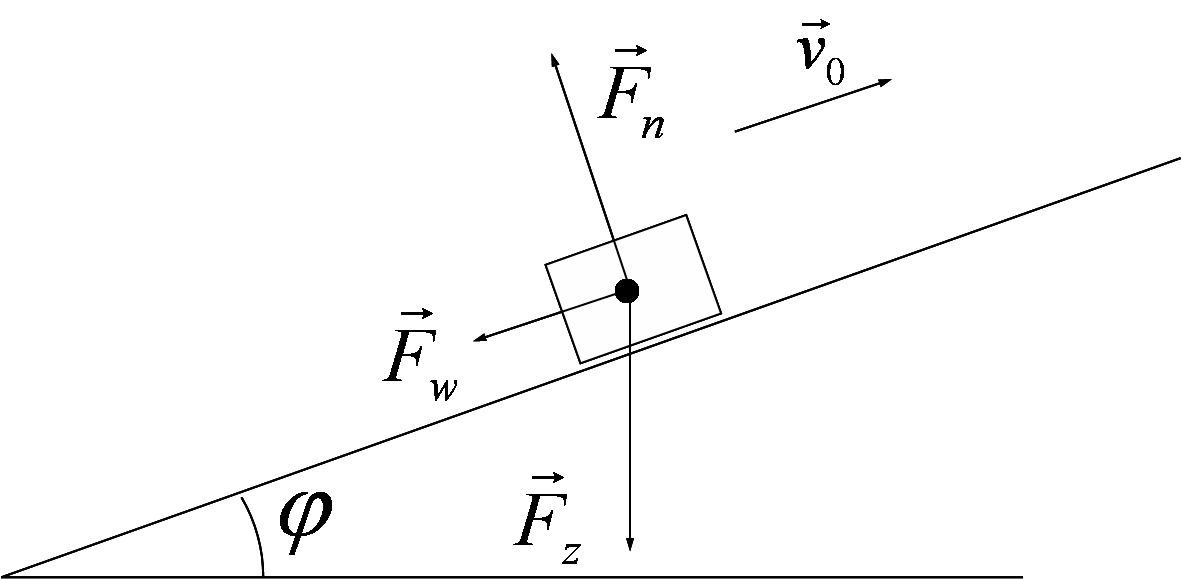
\includegraphics[width=0.49\textwidth,angle=0]{dyn/exercises/blok_helling_2}
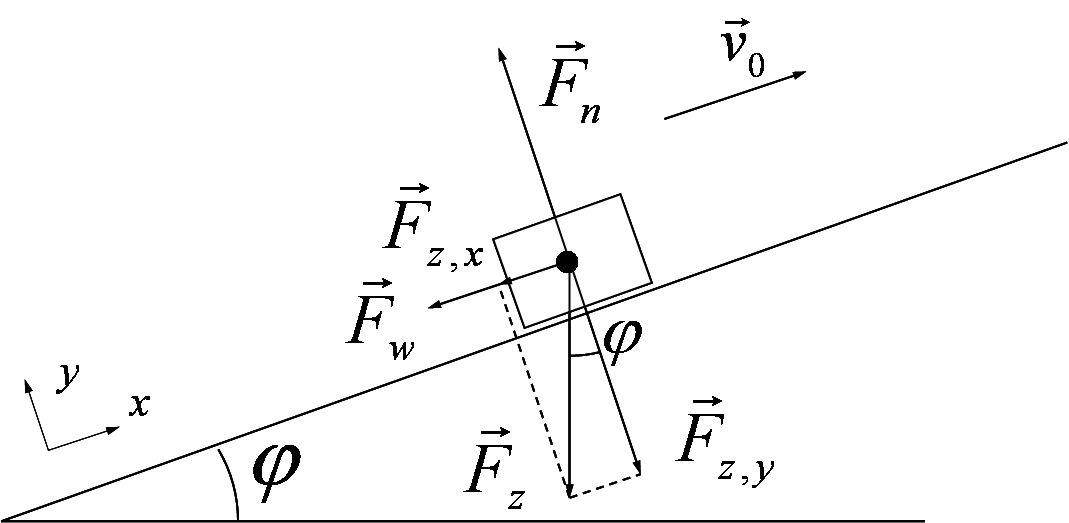
\includegraphics[width=0.49\textwidth, angle=0]{dyn/exercises/blok_helling_2componenten}
\end{flushright}
\end{figure}
$a=-\frac{F_w+mg\sin\varphi}{m}=-8,66\rm\,m/s^2$
\newline
$x=-\frac{v_0^2}{2a}=\frac{mv_0^2}{2(F_w+mg\sin\varphi)}=3,70\rm\,m$ %($t=0,92\rm\,s$) 
\newline
$F_{zx}>F_w$ zodat het blok terug naar beneden komt. 
\newline
$\mu=\frac{F_w}{mg\cos\varphi}=0,44$
\end{oplossing}



\end{exercise}

\begin{exercise} Een blok ligt op een helling. Bepaal de maximale hoek die de
helling kan maken met de horizontale zodat het blok n\'et niet in
beweging komt. De wrijvingsfactor is $\mu$.
\begin{oplossing}
\newline
We kiezen een assenstelsel met de $x$-as volgens de helling. De
zwaartekracht moeten we dan ontbinden in haar componenten.
\begin{eqnarray*}
\tan{\varphi}&=&\frac{F_{z,x}}{F_{z,y}}\\
&\Updownarrow&\\
F_{z,x}&=&F_{z,y}\tan{\varphi}\\
&=&F_n\tan{\varphi}\\
\end{eqnarray*}
Het blok is in rust zodat de $x$-component gelijk moet zijn aan de
wrij\-vings\-kracht. Omdat het blok nog net niet in beweging komt,
kunnen we de wrijvingskracht gelijkstellen aan $F_w=\mu F_n$. Dus:
\begin{eqnarray*}
F_w&=&F_n\tan{\varphi}\\
&\Downarrow&\\
\mu F_n&=&F_n\tan{\varphi}\\
&\Downarrow&\\
\mu&=&\tan{\varphi}
\end{eqnarray*}
De maximale hoek is ${\rm Bgtan\,}\mu$.
\end{oplossing}

\end{exercise}

\begin{exercise} Een steen wordt aan een touwtje in een horizontaal vlak rondgeslingerd met een snelheid die in grootte constant is. Heeft de steen een versnelling? Ondervindt de steen een resulterende kracht? Leg uit.


\end{exercise}

\begin{exercise} Een bestuurder van een auto met een massa van $1000~\rm kg$ rijdt aan een snelheid in grootte gelijk aan $10~\rm m/s$. Hij probeert een horizontale bocht, met een straal van $100~\rm m$ te nemen. De maximale wrijvingskracht tussen de banden en de baan is $900~\rm N$. Kan de auto deze bocht nemen of zal hij beginnen slippen?
\begin{oplossing}
\newline
\newline
De auto zal slippen in de bocht. Omdat we de snelheid en de straal kennen, kunnen we de versnelling van de gewenste cirkelbeweging berekenen. Met de tweede wet van Newton vinden we de (middelpuntzoekende) kracht nodig om deze versnelling te kunnen veroorzaken:
\begin{eqnarray*}
F&=&ma\\
&=&\frac{mv^2}{r}\\
&=&1000\rm\,N
\end{eqnarray*}
Dit is meer dan wat de grond maximaal op de wielen kan uitoefenen. De auto zal dus beginnen slippen.
\newline
\newline
Realiseer je dat de wrijvingskracht door de grond op de auto wordt uitgeoefend en de resulterende kracht vormt. Het is dan ook de middelpuntzoekende kracht. 
\begin{figure}[h]
\centering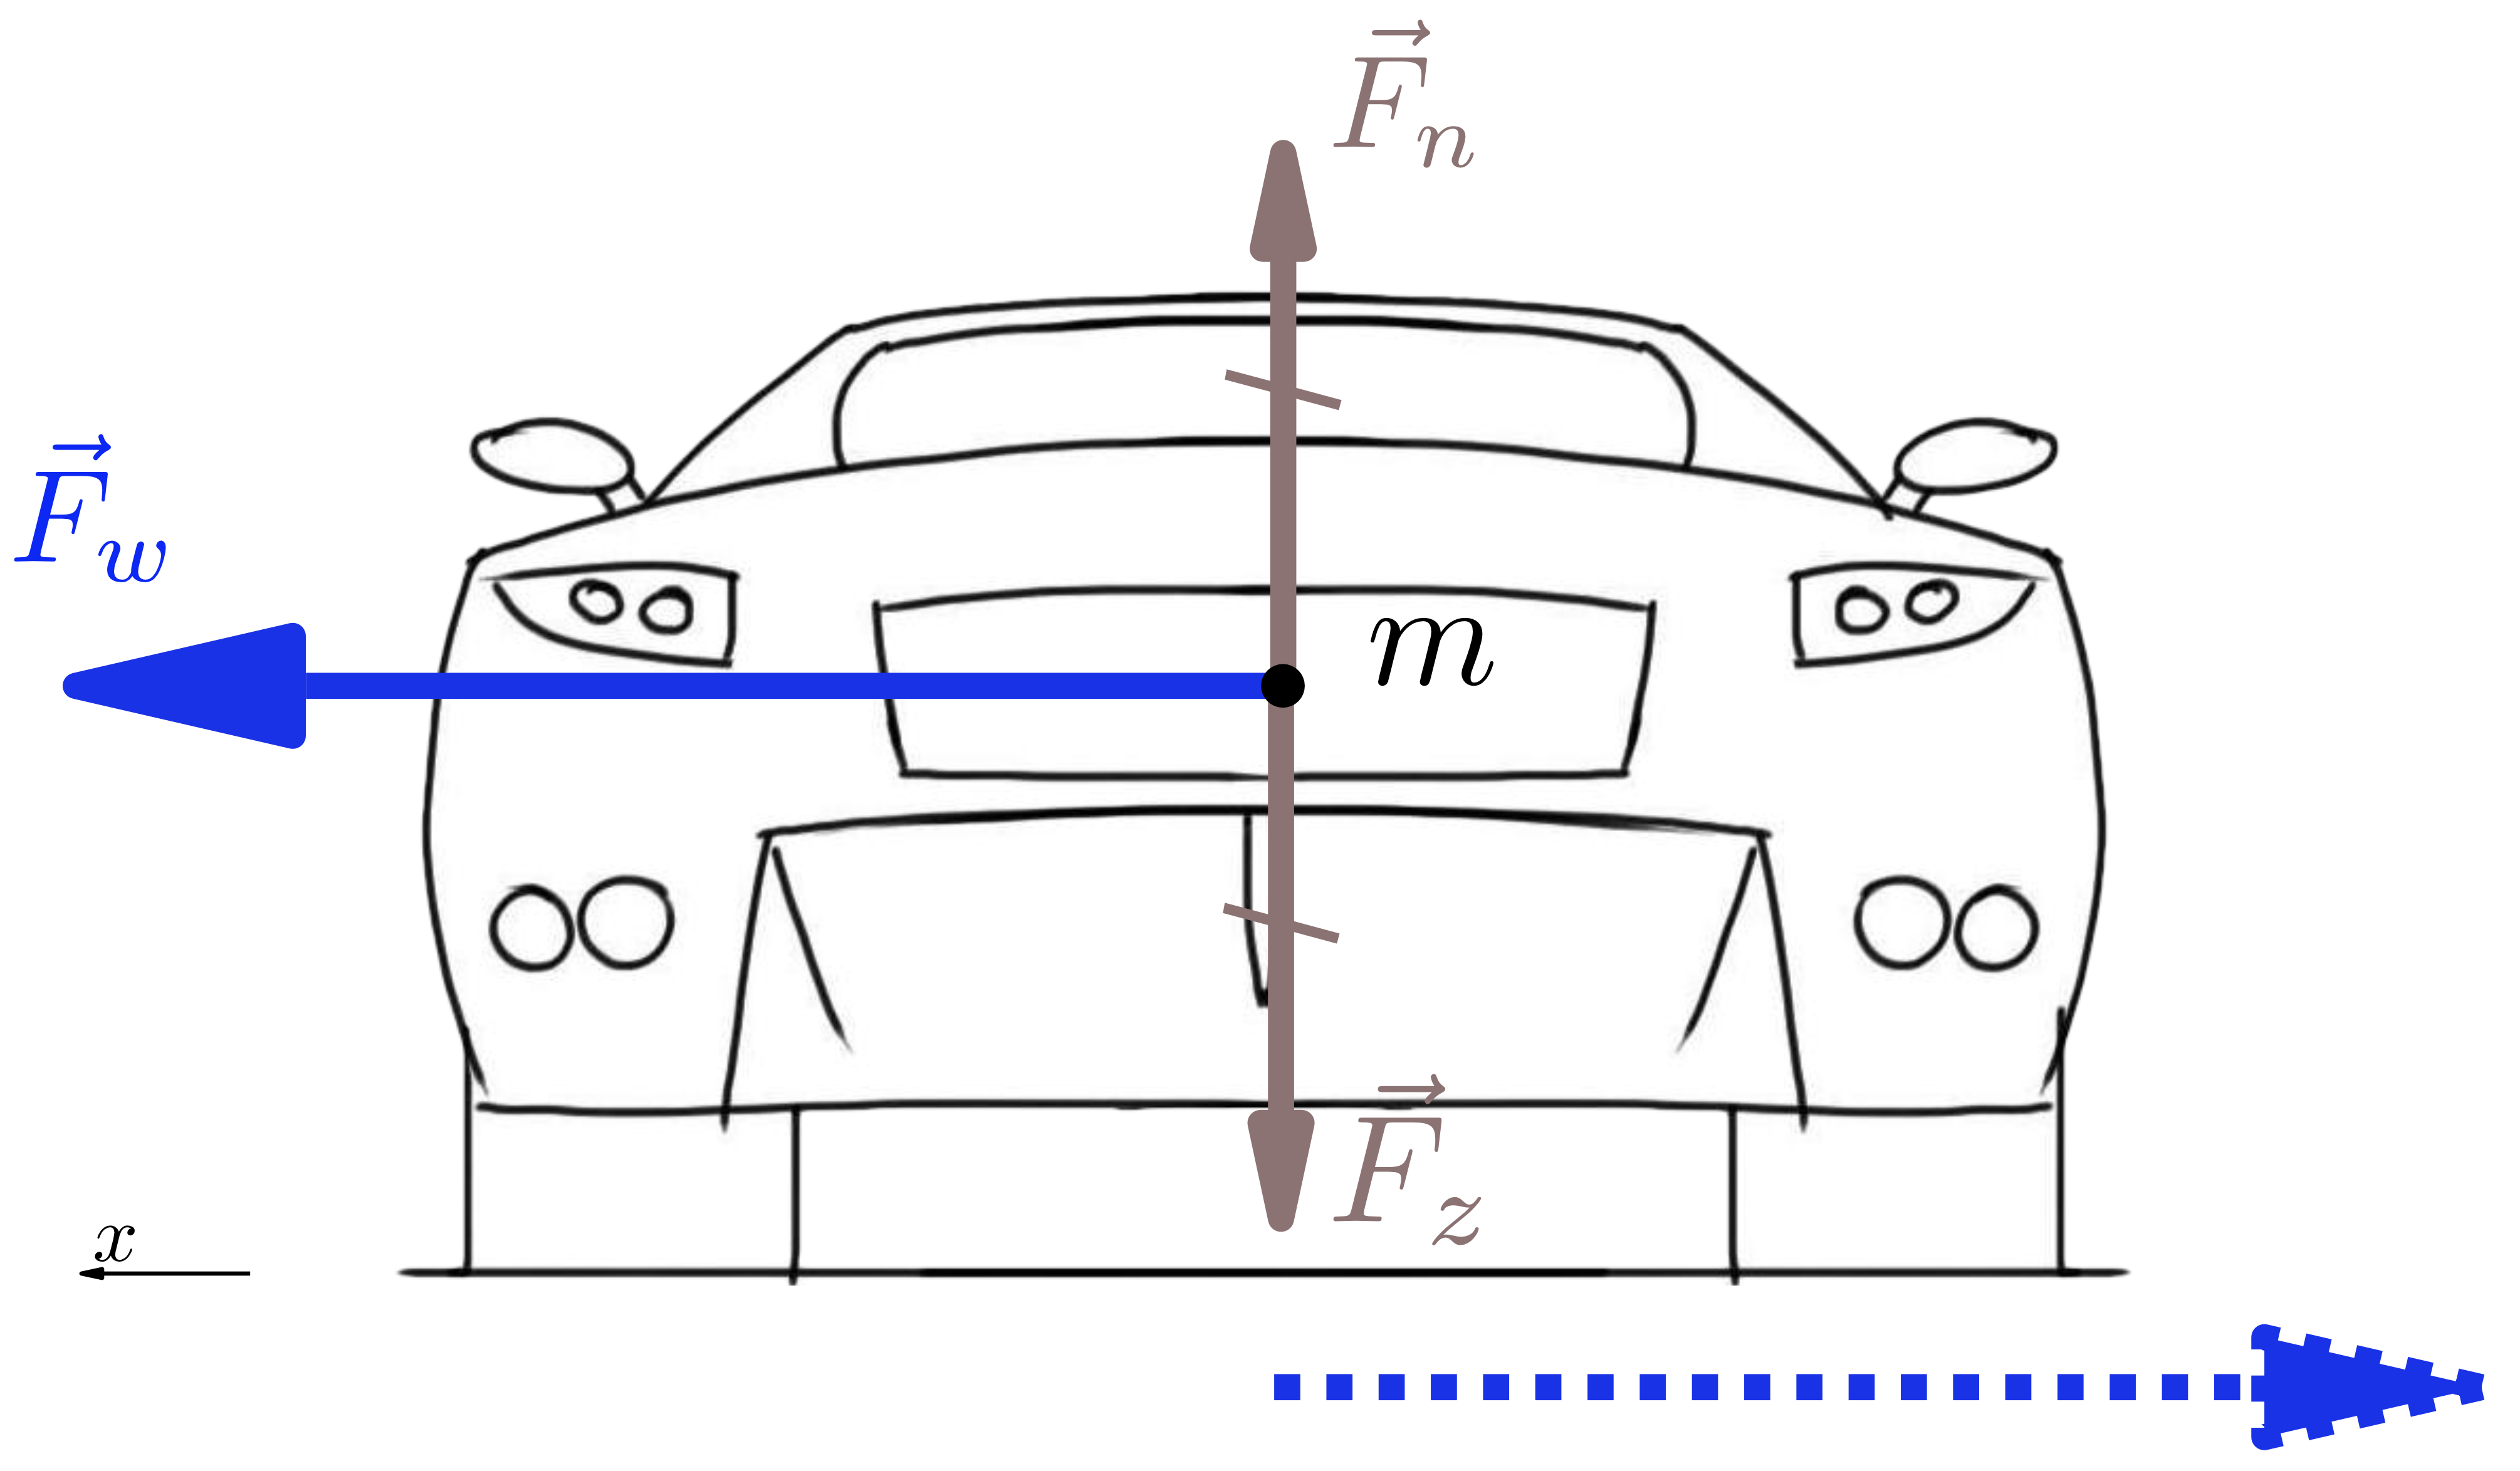
\includegraphics[width=0.5\textwidth, angle=0]{dyn/exercises/auto_bocht_horizontaal}
\end{figure}
De auto duwt met zijn wielen dwars ten opzichte van de snelheid tegen de grond en de grond duwt terug. In de figuur beweegt de auto het vlak van de tekening in en neemt de auto een bocht naar links (in de richting van de wrijvingskracht).
\end{oplossing}



\end{exercise}

\begin{exercise} Een cirkelvormige renbaan is onder een helling van $30^\circ$
gebouwd. De straal van de cirkel is $50~\rm m$. Met welke snelheid
moet een auto rijden om in de baan te blijven? Veronderstel dat de
baan spekglad is. 
\begin{oplossing}
\begin{figure}[h]
\centering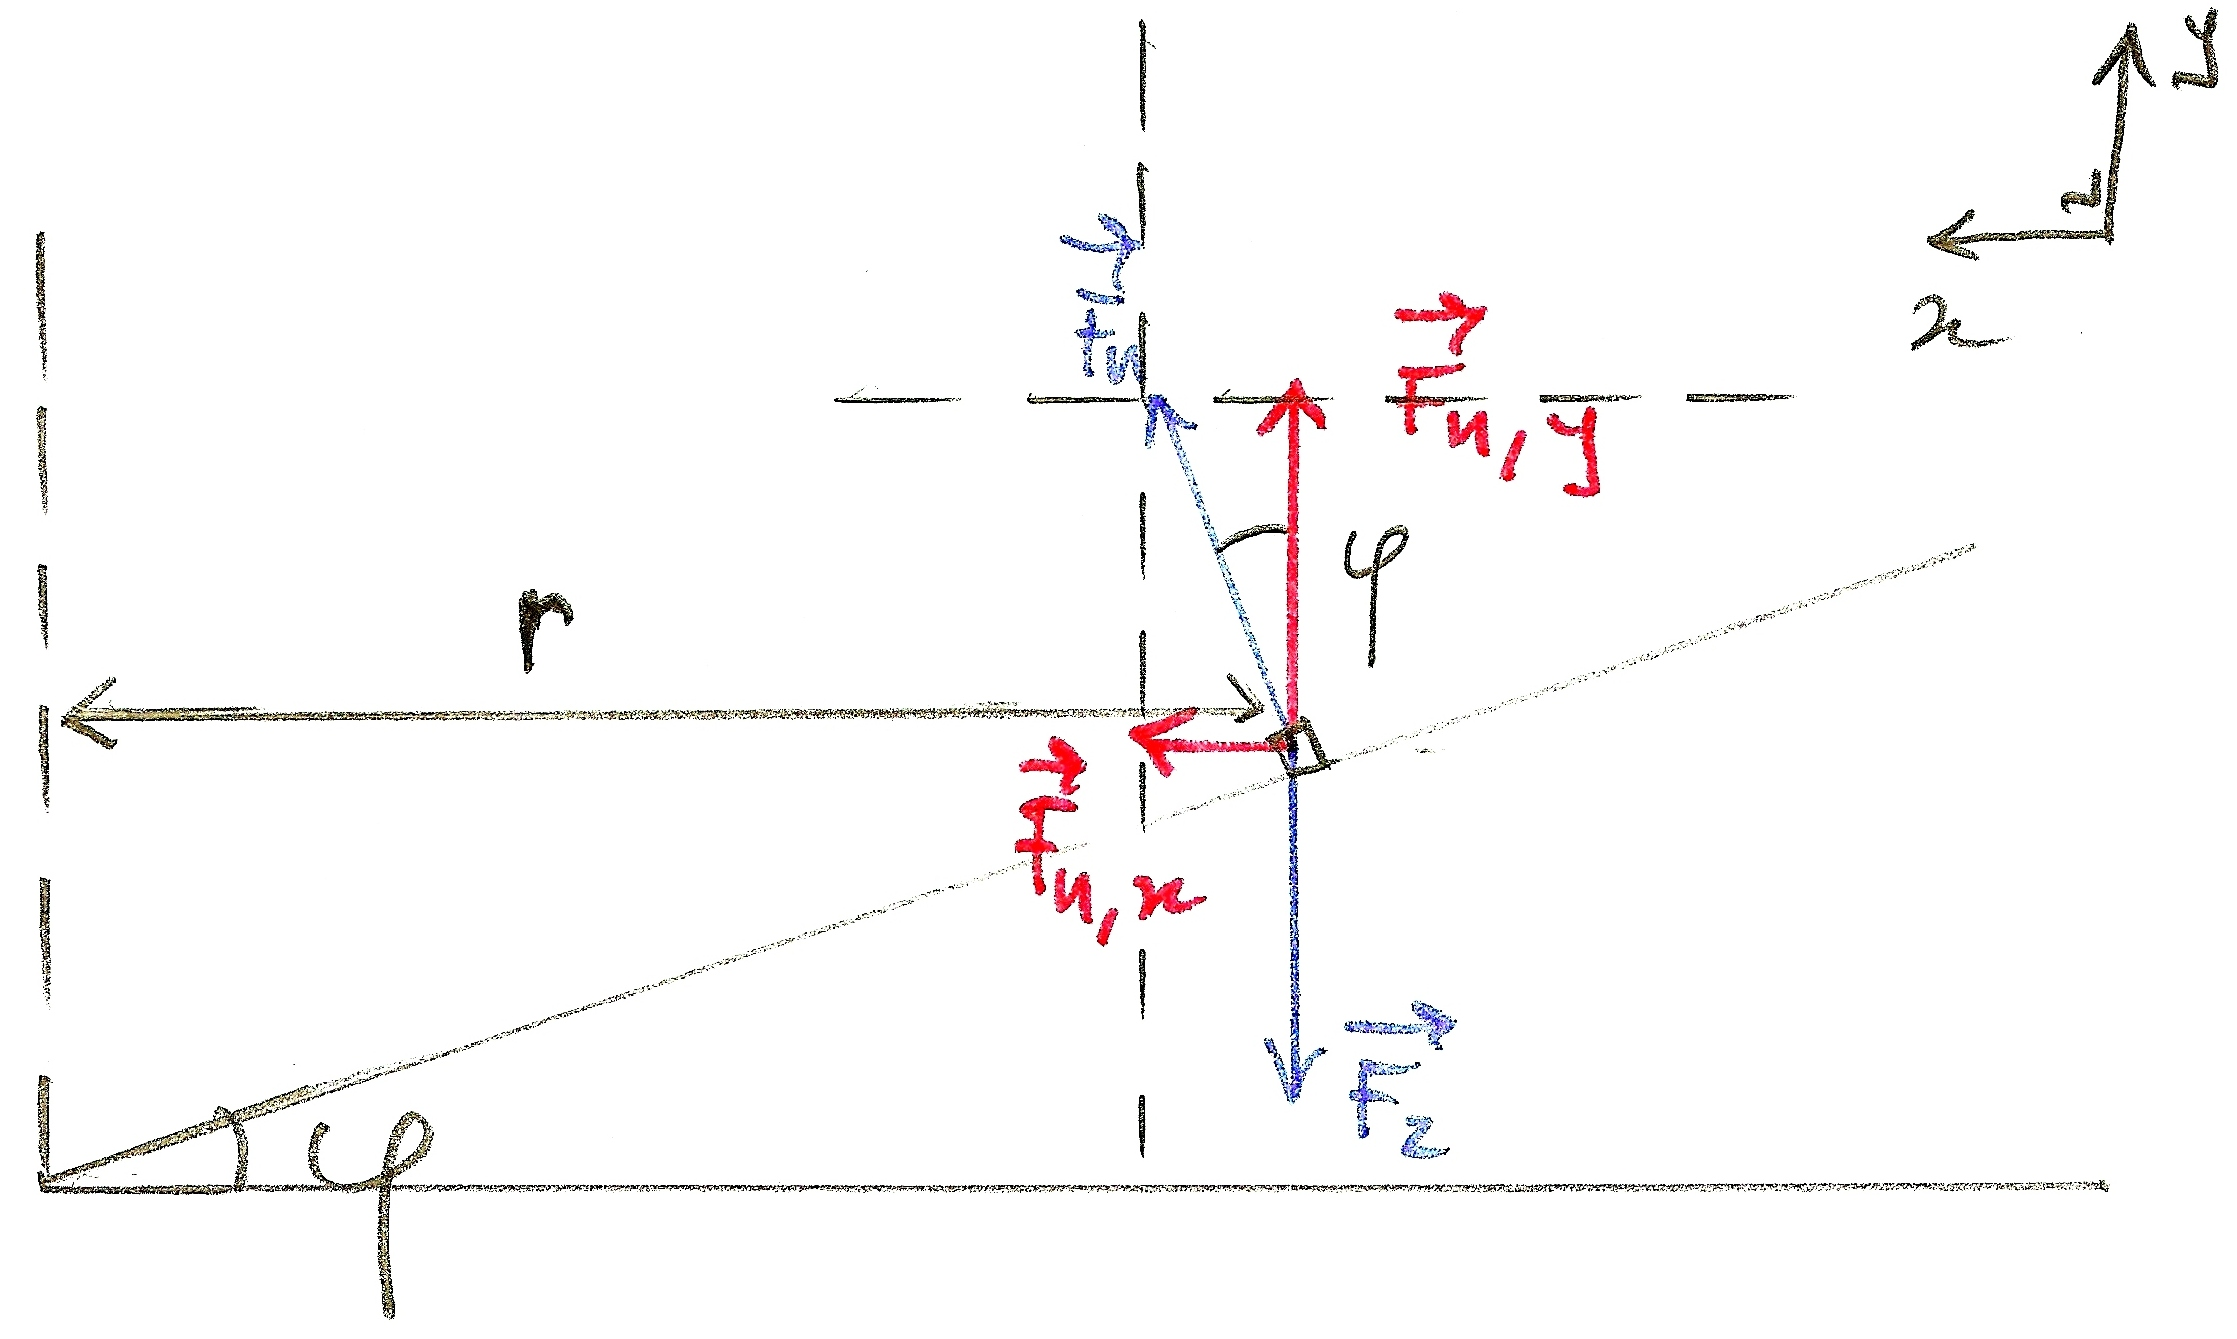
\includegraphics[width=0.6\textwidth, angle=0]{dyn/exercises/renbaan}
\end{figure}


\textit{gegeven}: $\varphi=30^\circ$\newline$r=50\rm\,m$

\textit{gevraagd:} $v$

\textit{oplossing:} De krachten die op de auto aangrijpen, zijn de zwaartekracht en de normaalkracht. In de $y$-richting is er geen versnelling omdat de auto in een horizontaal vlak beweegt. We kiezen dan ook een assenstelsel met de $y$-as verticaal geori\"enteerd. De $x$-as kunnen we in de richting van het centrum van de cirkel nemen. De $y$-component van de normaalkracht moet dus even groot zijn als de zwaartekracht. De $x$-component van de normaalkracht is dan ook de resulterende kracht en levert de middelpuntzoekende kracht. De $x$-component van de normaalkracht kunnen we m.b.v. de hoek en de zwaartekracht schrijven.
\newline
\newline
De $x$-component van de normaalkracht:
\begin{eqnarray*}
\tan{\varphi}&=&\frac{F_{n,x}}{F_{n,y}}\\
&\Updownarrow&\\
F_{n,x}&=&F_{n,y}\tan{\varphi}\\
&=&mg\tan{\varphi}
\end{eqnarray*}
We passen de tweede wet van Newton toe:
\begin{eqnarray*}
\vec{F}&=&m\vec{a}\\
&\Downarrow&\\
F_{n,x}&=&ma\\
mg\tan{\varphi}&=&\frac{mv^2}{r}\\
%&\Downarrow&\\
v&=&\sqrt{gr\tan{\varphi}}
\end{eqnarray*}
De gegevens invullen levert een snelheid van $17\rm\,m/s$.
\end{oplossing}

%\newpage


\end{exercise}

\begin{exercise} Op een draaitafel draait met een constante hoeksnelheid een grammofoonplaat. Twee muntstukken A en B zijn op zo'n plaats van het middelpunt van de draaitafel geplaatst dat zij nog net niet wegschuiven. Voor muntstuk A bedraagt de afstand tot de rotatieas dan $6\rm\,cm$ en voor B is het dan $12\rm\,cm$. $m_a$ en $m_b$ zijn de massa's van respectievelijk de muntstukken A en B. $\mu_a$ en $\mu_b$ zijn de wrijvingsfactoren tussen de muntstukken en de grammofoonplaat.
\newline
Welke gevolgtrekking m.b.t. de massa's en de wrijvingsfactoren is juist?
\newline
\newline
\begin{tabularx}{\textwidth}{*4{X}}
(a) $\displaystyle\mu_a=\frac{\mu_b}{2}$ & (b) $\displaystyle m_a=2m_b$ & (c) $\displaystyle m_a=\frac{m_b}{2}$ & (d)	$\displaystyle\frac{m_a}{\mu_a}=2\frac{m_b}{\mu_b}$
\end{tabularx}
\begin{oplossing}
Het juist antwoord is A. De wrijvingskracht tussen de muntjes en de
draaitafel moet voor de middelpuntzoekende kracht op de muntjes
zorgen. Als de muntjes nog n\'et niet wegschuiven, mogen we de
formule $F_w=\mu F_n$ voor de wrij\-vings\-kracht gebruiken. Dit
levert, met $F_n=F_z=mg$:
\begin{eqnarray*}
F&=&ma\\
&\Downarrow&\\
\mu mg&=&mr\omega^2\\
&\Downarrow&\\
\frac{\mu_a}{\mu_b}&=&\frac{r_a\omega^2}{g}\cdot\frac{g}{r_b\omega^2}\\
&=&\frac{r_a}{r_b}\\
&=&\frac{1}{2}
\end{eqnarray*}
\end{oplossing}

\end{exercise}

\begin{exercise} Een speelgoedwagentje beweegt in een horizontale cirkel met straal
$2l$ en heeft een tijd $T$ nodig om een volledige cirkel te
beschrijven. Dit kan omdat aan het wagentje een veer vastgemaakt is
.De lengte van de veer in niet uitgerekte toestand is $l$. Het
wagentje versnelt waarbij de straal van de beschreven cirkel gelijk
wordt aan $3l$.
\newline
De tijd die het wagentje nu nodig heeft om een volledige cirkel te
beschrijven is dan gelijk aan:
\begin{enumerate}
\item $T$
\item $\frac{3}{4}T$
\item $\sqrt{\frac{3}{4}}T$
\item $\sqrt{\frac{4}{3}}T$
\end{enumerate}
\begin{oplossing}
\textit{gegeven}
\begin{tabular}[t]{lcl}
$r$&=&$2l$\\
$r'$&=&$3l$\\
\end{tabular}

\textit{gevraagd}
\begin{tabular}[t]{ll}
$T'/T$
\end{tabular}

\textit{oplossing} De veerkracht zorgt voor de middelpuntzoekende kracht. We leiden hieruit een uitdrukking af voor de periode:
\begin{eqnarray*}
F&=&ma\\
&\Downarrow&\\
k\Delta l &=& mr\omega^2\\
&=&  mr\left(\frac{2\pi}{T}\right)^2\\
&\Updownarrow&\\
T^2&=&\frac{4\pi^2mr}{k\Delta l}
\end{eqnarray*}
De verhouding van het kwadraat van de periodes wordt dan:
\begin{eqnarray*}
\frac{T'^2}{T^2}&=&\frac{4\pi^2mr'}{k\Delta l'}\cdot\frac{k\Delta l}{4\pi^2mr}\\
&&\\
&=&\frac{3l(2l-l)}{(3l-l)2l}\\
&&\\
&=&\frac{3}{4}\\
&\Downarrow&\\
T'&=&\sqrt{\frac{3}{4}}\,T
\end{eqnarray*}
Het juiste antwoord is C.
\end{oplossing}





\end{exercise}

\begin{exercise} Waarom vliegt bij het afschieten van een kanonskogel, het kanon niet even ver achteruit als dat de kogel vooruit vliegt?


\end{exercise}

\begin{exercise} Moet een fietser, die op een horizontale weg eenparig rechtlijnig fietst, toch blijven trappen? Verklaar.

\end{exercise}

\begin{exercise} Een fietser met een massa van $60,2\rm\,kg$ rijdt op een rechte baan met een constante snelheid die $25,0\rm\,km/h$ bedraagt. Hoe groot is de inwerkende resulterende kracht? 
\begin{oplossing}
De resulterende kracht is 0. De eerste wet van Newton zegt dat een voorwerp maar een ERB kan uitvoeren indien de resulterende kracht erop nul is. Zou er een van nul verschillende kracht op de fietser inwerken dan krijgt hij een versnelling. Je moet blijven trappen om een kracht te genereren die even groot is als de wrijvingskracht.
\end{oplossing}

\end{exercise}

\begin{exercise} Kareltje is net vier jaar geworden en vindt dat hij groot genoeg is om mama te helpen wanneer zij hem naar school brengt met de fiets. Vanuit zijn kinderstoel achterop zal hij mama flink in de rug duwen. Wat ziet Kareltje over het hoofd? 

\end{exercise}

\begin{exercise} Geef aan of de volgende uitspraken waar of vals zijn. Licht je antwoord toe.
\begin{enumerate}
\item Als een lichaam niet versnelt dan kan er geen kracht op werken. 
\item Bij een parachutist is de zwaartekracht even groot als de weerstandskracht -- die hij ondervindt van de lucht -- wanneer hij met zijn parachute met een constante snelheid naar beneden daalt. 
%\item Wanneer je een kilo meel aan de evenaar koopt krijg je minder meel dan wanneer je een kilo meel op de noordpool zou kopen.
\end{enumerate}


\end{exercise}

\begin{exercise} Toon aan dat de remweg van een remmende auto omgekeerd
evenredig is met de wrijvingsfactor. Veronderstel dat de wielen
glijden over het wegdek.

\end{exercise}

\begin{exercise} Als we de `effectieve zwaartekracht' in een centrifuge willen vergroten, wat is dan beter: de straal verdubbelen of de hoeksnelheid verdubbelen?

\end{exercise}

\begin{exercise} Stel dat we een emmer met water aan een touw rondslingeren in een verticaal vlak zodanig dat het water niet uit de emmer valt. Neemt het (schijnbaar) gewicht van het water in de emmer toe wanneer we de emmer met een grotere snelheid laten ronddraaien? Leg uit.

\end{exercise}

\begin{exercise} Er wordt wel gezegd dat in een wasmachine water uit het wasgoed wordt verwijderd doordat de centrifugaalkracht het water naar buiten trekt. Is dit correct? Leg uit.

\end{exercise}

\begin{exercise} Verklaar hoe een fietser op een horizontaal wegdek een bocht kan nemen. Bepaal ook de maximale snelheid waarmee je door een bocht met straal $r$ kan gaan, als de wrijvingsfactor tussen de weg en de banden $\mu$ is.

\end{exercise}

\begin{exercise} Geef de formule voor de grootte van de middelpuntzoekende kracht.

\end{exercise}

\begin{exercise} Welk punt heeft de grootste versnelling: een punt op de buitenrand
van een ronddraaiende cd, of een punt op de helft van de straal van
een cd die met een tweemaal zo grote hoeksnelheid ronddraait? Toon
je antwoord aan.

\end{exercise}





\subsection{Vraagstukken}


\begin{exercise} Om een ongeval te vermijden, drukt een bestuurder van een auto zijn remmen volledig in. Na een remspoor van \SI{90}{m} komt hij tot stilstand. De wrijvingsfactor tussen de wielen en de weg is gelijk aan \SI{0,500}{}. Bepaal de snelheid die hij voor het remmen had.

\begin{oplossing}
$v_0=\sqrt{2\mu gx}=\SI{29,71}{m/s}=\SI{107}{km/h}$
\end{oplossing}

\end{exercise}

\begin{exercise} Een massa van $50,0~\rm g$ wordt door een horizontale kracht van $0,065~\rm N$ voortbewogen. Hij legt
onder de werking van deze kracht en de wrij\-vings\-kracht vanuit de rusttoestand in $10,0~\rm s$ op een rechte baan een afstand af van $40,7~\rm m$. Hoe groot zijn de wrijvingskracht en de wrijvingsfactor?
\begin{oplossing}
\textit{gegeven}
\begin{tabular}[t]{lcl}
$m$ &$=$& $50,0\cdot10^{-3}~\rm kg$\\
$F$ &$=$& $0,065~\rm N$\\
$t$ &$=$& $10,0~\rm s$\\
$x$ &$=$& $40,7~\rm m$\\
\end{tabular}

\textit{gevraagd}
$F_w$, $\mu$

\textit{oplossing}
Uit de vergelijkingen voor een EVRB vinden we de versnelling:
\begin{eqnarray}
x &=& x_0+v_0t+\frac{1}{2}at^2\nonumber\\
&\Downarrow& \nonumber\\
a &=&\frac{2x}{t^2}\label{versn_a}
\end{eqnarray}
Volgens de $x$-as samen met (\ref{versn_a}) geldt:
\begin{eqnarray}
F-F_w&=&ma\nonumber\\
&\Downarrow& \nonumber\\
F_w &=& F-m\frac{2x}{t^2}\label{F_w}\\
&=& 65\cdot10^{-3}~{\rm N}-50,0\cdot10^{-3}~{\rm kg}\frac{2\cdot40,7~{\rm m}}{{10,0~{\rm s}}^2}\nonumber\\
&=& 0,024~\rm N\nonumber
\end{eqnarray}
Uit vergelijking (\ref{F_w}) en $F_w=\mu F_n=\mu mg$ volgt:
\begin{eqnarray*}
\mu &=& \frac{F}{mg}-\frac{2x}{gt^2}\\
&=& 0,050
\end{eqnarray*}
\end{oplossing}

\end{exercise}

\begin{exercise} Toon aan dat de remweg van een remmende auto omgekeerd
evenredig is met de wrijvingsfactor. Veronderstel dat de wielen
glijden over het wegdek.
%Zie oplossing opdracht 33 HB p. 111, hier vonden we (\ref{remvgl}):
\begin{oplossing}
\begin{eqnarray*}
\mu&=&\frac{v_0^2}{2gx}\\
&\Updownarrow&\\
x&=&\frac{v_0^2}{2g\mu}
\end{eqnarray*}
De remweg $x$ is dus omgekeerd evenredig met de wrijvingsfactor $\mu$.
\end{oplossing}

\end{exercise}

\begin{exercise} Een auto rijdt op een horizontale baan met een snelheid van
$108\rm\,km/h$. Als hij plots moet remmen, wat is dan zijn kleinste
remafstand in de veronderstelling dat de wielen schuiven over het
wegdek en de wrijvingsfactor tussen de wielen en de weg gelijk is
aan $0,500$?
%Zie oplossing opdracht 33 HB p. 111, hier vonden we (\ref{remvgl}):
\begin{oplossing}
\begin{eqnarray*}
\mu&=&\frac{v_0^2}{2gx}\\
&\Updownarrow&\\
x&=&\frac{v_0^2}{2g\mu}\\
&=&\frac{(30\rm\,m/s)^2}{2\cdot9,81\rm\,m/s^2\cdot0,500}\\
&=&91,7\rm\,m
\end{eqnarray*}
\end{oplossing}


\end{exercise}

\begin{exercise} Een massa van $10,0~\rm kg$ is aan touwen opgehangen zoals in de figuur. De hoek is $\theta=60^\circ$. Bepaal de spankrachten $F_1,~F_2$ en $F_3$ in het touw.
\begin{figure}[h]
\begin{center}
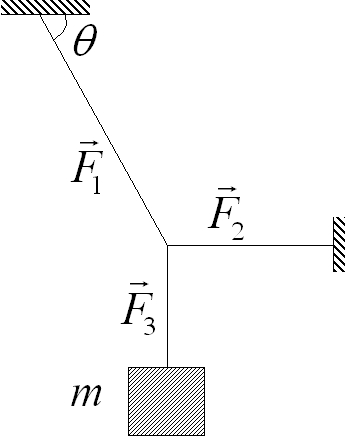
\includegraphics[width=.4\textwidth]{dyn/exercises/massa_aan_touw}
\end{center}
\end{figure}




\end{exercise}

\begin{exercise} Een zak cement met massa $m$ hangt aan drie touwen zoals weergegeven op de figuur. Twee van de drie touwen maken een hoek $\theta_1$, respectievelijk $\theta_2$ met de horizontale. Het geheel is in rust.
\begin{enumerate}
\item Bewijs dat de grootte van de spankracht in het linkertouw te berekenen is uit:
\[
F_1=\frac{mg\cos{\theta_2}}{\sin{(\theta_1+\theta_2)}}
\]
\item Als de massa van de cement $20,4\rm\,kg$ bedraagt, $\theta_1=10,0^\circ$ en $\theta_2=25,0^\circ$ hoe groot zijn dan de spankrachten in de drie touwen?
\end{enumerate}
\begin{oplossing}
\begin{enumerate}
\item In de horizontale $x$-richting is er geen versnelling zodat volgens de tweede wet van Newton de componenten van de krachten in deze rich\-ting elkaar moeten opheffen:
\begin{eqnarray}
\sum_{i=1}^3F_{i,x}&=&ma_x\nonumber\\
&\Updownarrow&\nonumber\\
F_{1,x}+F_{2,x}+F_{3,x}&=&ma_x\nonumber\\
&\Downarrow&\nonumber\\
-F_1\cos{\theta_1}+F_2\cos{\theta_2}+0&=&0\label{cement1}
\end{eqnarray}
Ook in de verticale $y$-richting moeten de krachten elkaar opheffen,
ook hier is er geen versnelling:
\begin{eqnarray}
F_1\sin{\theta_1}+F_2\sin{\theta_2}-mg&=&0\label{cement2}
\end{eqnarray}
We hebben twee vergelijkingen met twee onbekende krachten. We lossen
op naar $F_1$:
\begin{eqnarray}
(\ref{cement1})&\Leftrightarrow&F_2=\frac{F_1\cos{\theta_1}}{\cos{\theta_2}}\label{cement3}\\
(\ref{cement2})&\Leftrightarrow&F_2=\frac{mg-F_1\sin{\theta_1}}{\sin{\theta_2}}\nonumber
\end{eqnarray}
Deze uitdrukkingen aan elkaar gelijk stellen levert:
\begin{eqnarray*}
F_1\cos{\theta_1}\sin{\theta_2}&=&mg\cos{\theta_2}-F_1\sin{\theta_1}\cos{\theta_2}\\
&\Updownarrow&\\
F_1(\sin{\theta_1}\cos{\theta_2}+\cos{\theta_1}\sin{\theta_2})&=&mg\cos{\theta_2}\\
&\Updownarrow&\\
F_1&=&\frac{mg\cos{\theta_2}}{\sin{(\theta_1+\theta_2)}}
\end{eqnarray*}
\item Deze formule invullen in (\ref{cement3}) levert:
\begin{eqnarray*}
F_2&=&\frac{mg\cos{\theta_1}}{\sin{(\theta_1+\theta_2)}}
\end{eqnarray*}
\end{enumerate}
\end{oplossing}


\end{exercise}

\begin{exercise} Bereken de versnelling van het systeem in de figuur. De dynamische wrijvingsfactor is $\mu$ en het touw heeft een verwaarloosbare massa zodat de spankracht in het touw overal hetzelfde is. 
%figuur = blokken_op_helling.bmp


\end{exercise}

\begin{exercise} Drie voorwerpen zijn aan elkaar verbonden met touwtjes. De wrij\-vings\-factor tussen de tafel en het erop liggend voorwerp $V$ is $\mu$.
\begin{figure}[h]
\begin{center}
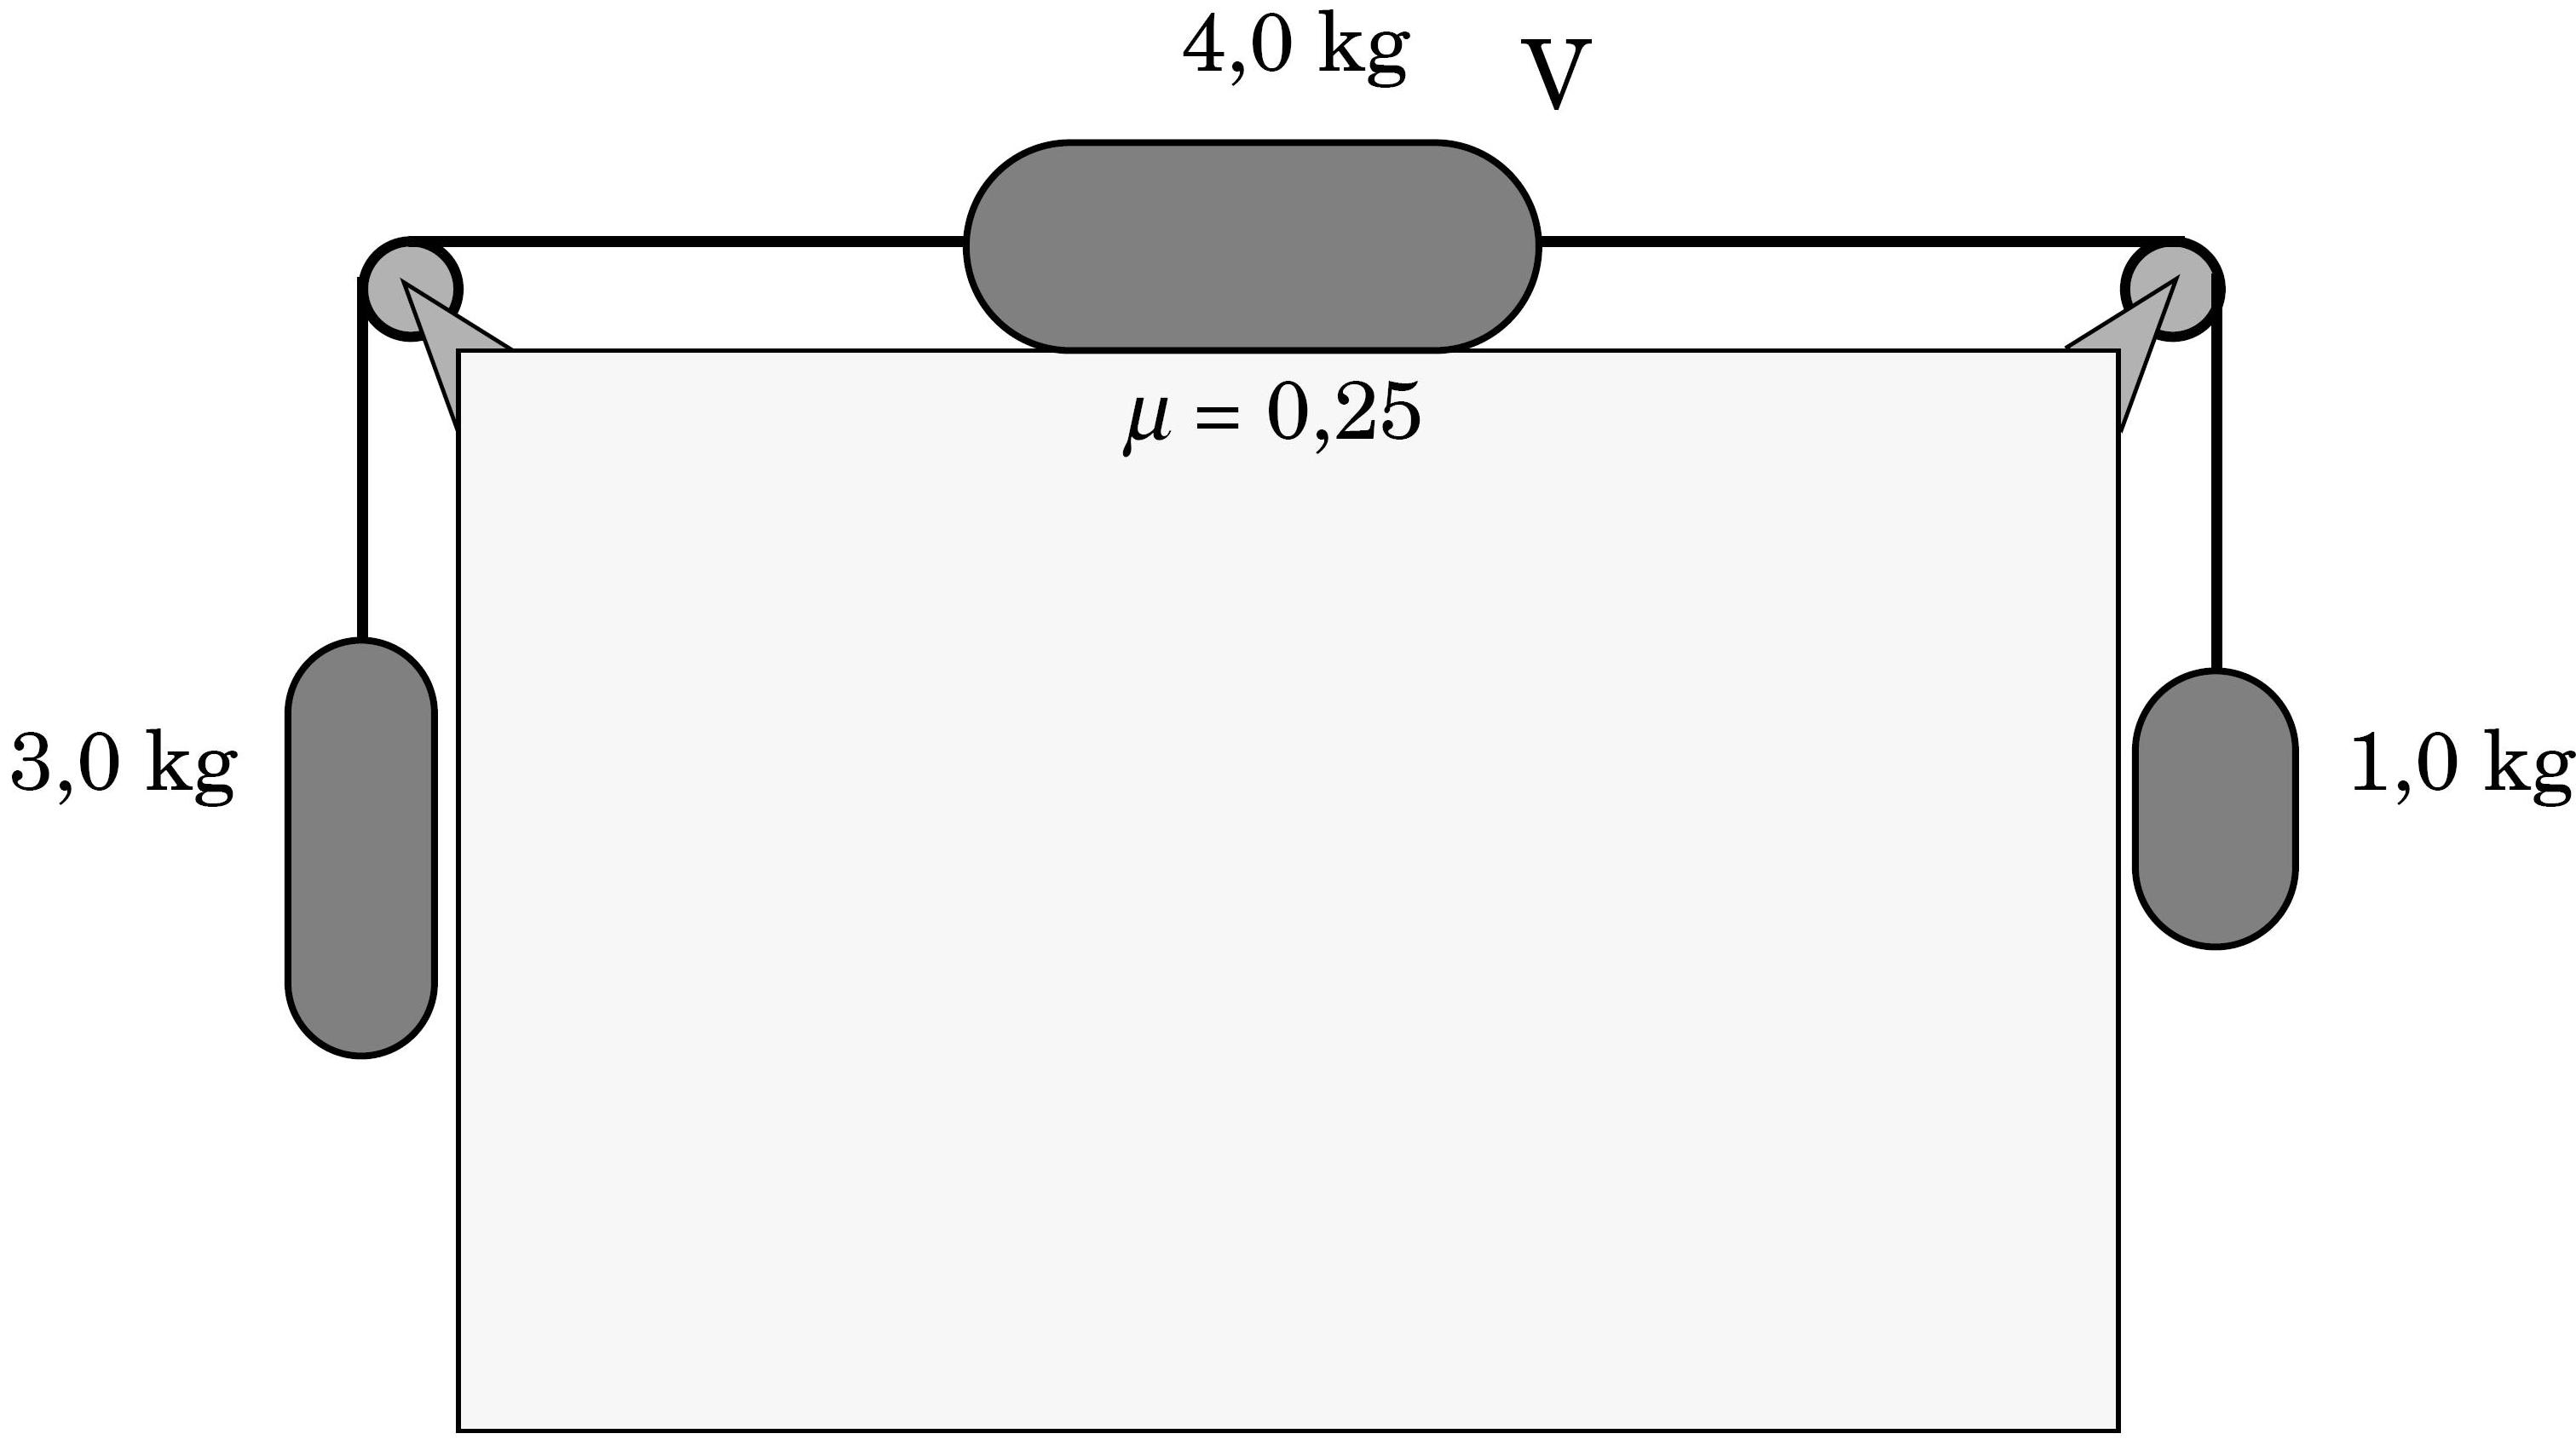
\includegraphics[width=0.6\textwidth ,angle=0]{dyn/exercises/drie_voorwerpen}
\end{center}
\end{figure}
Veronderstel dat er geen wrijving is in de katrollen en dat de massa van de katrollen te verwaarlozen is. Bepaal de versnelling van het voorwerp. \footnote{Bron: 16de VFO 2004}
\begin{oplossing}
\newline
Om de versnelling van het voorwerp te vinden kunnen we de tweede wet van Newton toepassen op de drie massa's. We tekenen de krachtendiagrammen op elk van de massa's (zie figuur). 
\begin{figure}[h]
\begin{center}
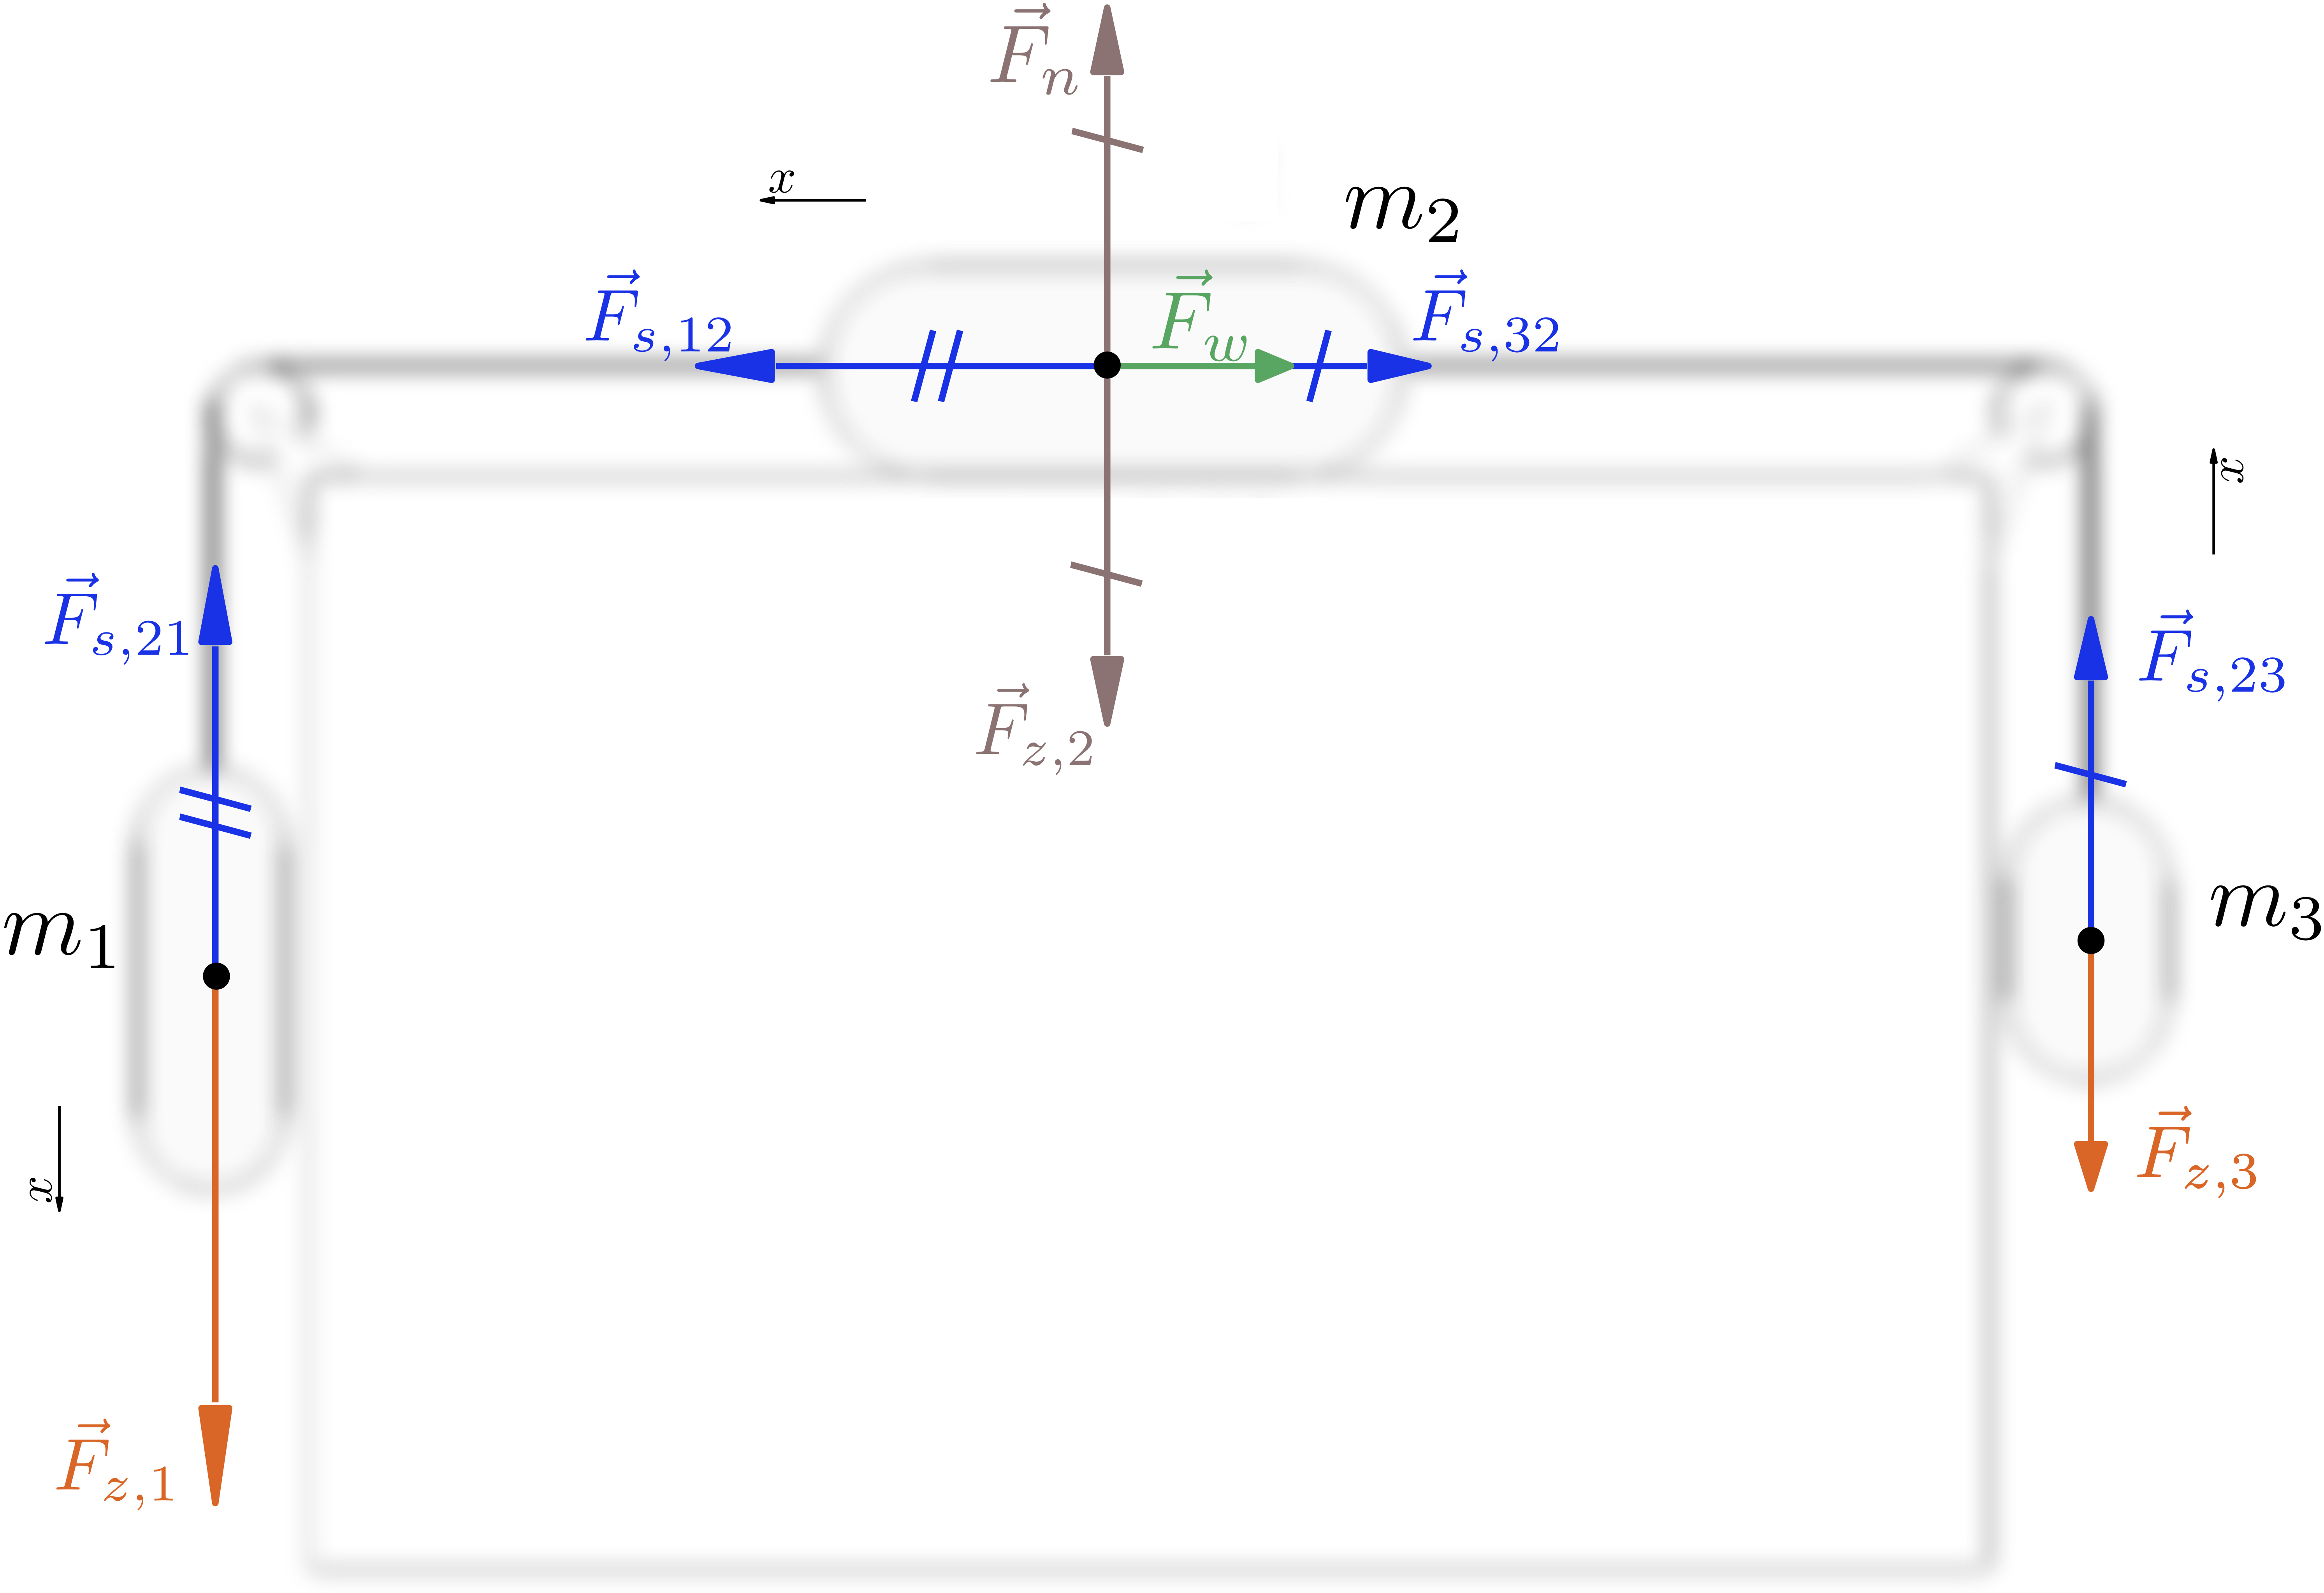
\includegraphics[width=0.73\textwidth ,angle=0]{dyn/exercises/drie_voorwerpen_krachten}
\end{center}
\end{figure}

Voor $m_1$ vinden we, met de keuze van de $x$-as verticaal naar beneden:
\begin{eqnarray}
F_{z,1}-F_{s,21}=m_1a\label{m_1}
\end{eqnarray}
Voor $m_3$ vinden we, met nu de keuze van de $x$-as verticaal naar boven:
\begin{eqnarray}
F_{s,23}-F_{z,3}=m_3a\label{m_3}
\end{eqnarray}
Voor $m_2$ vinden we, met de keuze van de $x$-as horizontaal naar links:
\begin{eqnarray}
F_{s,12}-F_w-F_{s,32}=m_2a\label{m_2}
\end{eqnarray}
Volgens de derde wet van Newton kunnen we de overeenkomstige spankrachten aan mekaar gelijk stellen: $F_{s,21}=F_{s,12}$ en $F_{s,32}=F_{s,23}$. Samen met $F_w=\mu F_n$ en $F_z=ma$ hebben we drie vergelijkingen en drie onbekenden. Oplossen naar de versnelling levert:
\begin{eqnarray*}
a=\frac{m_1-m_2-\mu m_3}{m_1+m_2+m_3}g=1,226\rm\,m/s^2
\end{eqnarray*}

Realiseer je dat de keuze van de $x$-as bij het bepalen van de componenten van de krachten de tekens bepalen van die componenten -- en ook die van de versnelling. Als je bijvoorbeeld tweemaal $a$ schrijft (in vergelijking (\ref{m_1}) en (\ref{m_3})) moet het ook effectief over dezelfde versnelling gaan, en niet over versnellingen die elkaars tegengestelde zijn. Met de $x$-as verticaal naar beneden geori\"enteerd voor $m_1$, zal de versnelling voor $m_1$ positief zijn als de massa naar beneden versnelt (wat hij doet; $m_1>m_3$). Voor $m_3$ moet je dan de $x$-as verticaal omhoog kiezen, wil je dat $a$ evenzeer positief is of dus dezelfde betekenis heeft.
\newline
\newline
Zie ook dat uit vergelijking (\ref{m_1}) volgt dat $m_1$ niet met de zwaartekracht aan $m_2$ trekt! De massa $m_1$ versnelt, waarvoor een resulterende kracht nodig is. 
\end{oplossing}



\end{exercise}

\begin{exercise} Een last van 1000 N hangt aan een kabel van $5,00\rm\,m$
lengte. Deze last wordt door een horizontale kracht $2,00\rm\,m$
zijwaarts uit zijn verticale stand getrokken.
\begin{enumerate}
    \item Bepaal de kracht waarmee zijwaarts aan de last werd
    getrokken.
    \item Bepaal de kracht waaraan het touw minimaal moet kunnen
    weerstaan zonder te breken.
\end{enumerate}


\end{exercise}

\begin{exercise} Als een persoon in vrije val ten gevolge van de
wrijvingskracht met de lucht valt met een maximumsnelheid van
ongeveer $240\rm\,km/h$ en deze wrijvingskracht is recht evenredig
met het kwadraat van de snelheid, bepaal dan deze
evenredigheidsconstante (= de wrijvinfsco\"effici\"ent). De persoon
heeft een massa van $66\rm\,kg$.


\begin{oplossing}
    \begin{itemize}
\item[24 p.72]Misschien eerst ter verduidelijking: de aangeduide kracht kan bijvoorbeeld worden uitgeoefend door een gewicht dat aan punt $A$ is opgehangen. Om de gevraagde krachten te vinden, kunnen we de gegeven kracht ontbinden. We kunnen haar beschouwen als samengesteld uit twee krachten. Namelijk de kracht op de staaf uitgeoefend ($\vec{F}_{ab}$, de staaf ondersteunt punt $A$) en de kracht waarmee aan het touw wordt getrokken ($\vec{F}{ac}$, het touw voorkomt dat $A$ naar beneden zou vallen zodat m.a.w. het punt aan het touw moet trekken).
    \begin{figure}[h]
    \centering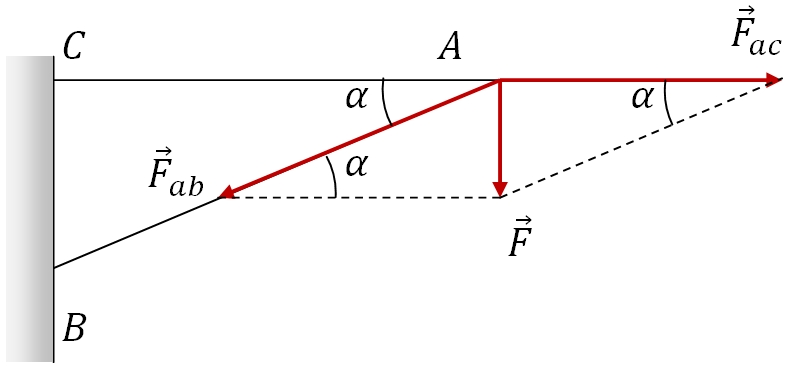
\includegraphics[width=0.7\textwidth]{dyn/exercises/24p72_fig}
    \end{figure}

    Voor $F_{ab}$ geldt:
    \begin{eqnarray*}
    \sin{\alpha}&=&\frac{F}{F_{ab}}\\
    &\Updownarrow&\\
    F_{ab}&=&\frac{F}{\sin{\alpha}}=\frac{1500\rm\,N}{\frac{1}{2}}=3,00\cdot10^3\rm\,N
    \end{eqnarray*}
    Voor $F_{ac}$ geldt:
    \begin{eqnarray*}
    F_{ac}&=&\frac{F}{\tan{\alpha}}=\frac{1500\rm\,N}{\frac{\sqrt{3}}{3}}=2,60\cdot10^3\rm\,N
    \end{eqnarray*}

\item[25 p.72]De zwaartekracht werkt verticaal naar beneden, grijpt aan op de massa en wordt door de aarde uitgeoefend. Ook de spankracht werkt op de massa. Deze wordt door het touw op de massa uitgeoefend. Ze is altijd volgens het touw gericht. Naast de wrijvingskracht die we hier buiten beschouwing laten, zijn dit de enige twee krachten die op de slingerende massa werken.

\item[27 p.73]De versnelling die een voorwerp met massa $m$ krijgt als gevolg van een kracht $F$, is volgens de tweede wet van Newton gelijk aan $a=\frac{F}{m}$ zodat:
\begin{eqnarray*}
v=at=\frac{Ft}{m}=10\rm\,m/s
\end{eqnarray*}

\item[29 p.73]Uit de formules voor een EVRB kunnen we een uitdrukking voor de vertraging vinden (zie voor de uitwerking de oplossingen van vraagstukken die we maakten in de kinematica):
\[
a=-\frac{v_0^2}{2x}
\]
Om deze vertraging te kunnen realiseren is volgens de tweede wet van Newton een kracht nodig gelijk aan:
\begin{eqnarray*}
F=ma=-m\frac{v_0^2}{2x}=-37500\rm\,N
\end{eqnarray*}
Het minteken slaat op het feit dat de kracht tegengesteld is aan de snelheid die met de keuze van de $x$-as mee is. De grootte van de kracht is dan de uitdrukking zonder het minteken.
\end{itemize}
\end{oplossing}

\begin{oplossing}
    \begin{itemize}

\item [36 p.112]
Het juist antwoord is B. $v_{max}=\sqrt{\mu rg}$ dus $v_{max}\sim\sqrt{r}$.

\item [37 p.112]
$v_{max}\sim\sqrt{r}$ dus moeten we $v_{max}$ uitzetten tegen
$\sqrt{r}$.
    \end{itemize}
\end{oplossing}



\end{exercise}

\begin{exercise} Een blokje op een wrijvingsloze tafel beschrijft een ECB doordat het vastgemaakt is aan een koordje dat door een
gaatje in de tafel gaat en waaraan een massa is verbonden die door
de zwaartekracht naar beneden wordt getrokken.
\begin{figure}[h]
\begin{center}
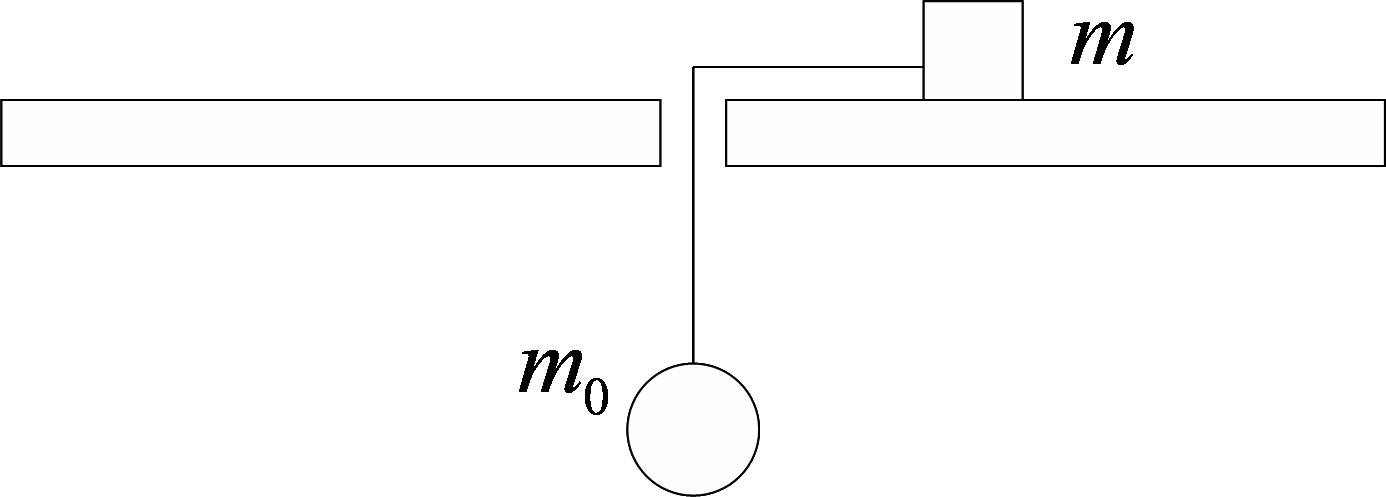
\includegraphics[width=0.4\textwidth, angle=0]{dyn/exercises/massa_op_tafel}
\end{center}
\end{figure}
\begin{enumerate}
\item Welke kracht levert de middelpuntzoekende kracht?
\item Kan voor cirkelbewegingen met een verschillende straal de
middelpuntzoekende kracht veranderen van grootte?
\item Hoe heb je proefondervindelijk geconstateerd dat de frequentie
voor verschillende stralen verschillend is?
\end{enumerate}

\end{exercise}

\begin{exercise} Een blokje op een wrijvingsloze tafel beschrijft een ECB met straal $r$ en snelheid $v$ doordat het vastgemaakt is aan een koordje dat door een gaatje in de tafel gaat en waaraan een massa is verbonden die door de zwaartekracht naar beneden wordt getrokken. Als de straal 2 maal groter wordt, hoeveel maal groter wordt dan de snelheid?
\begin{figure}[h]
\begin{center}
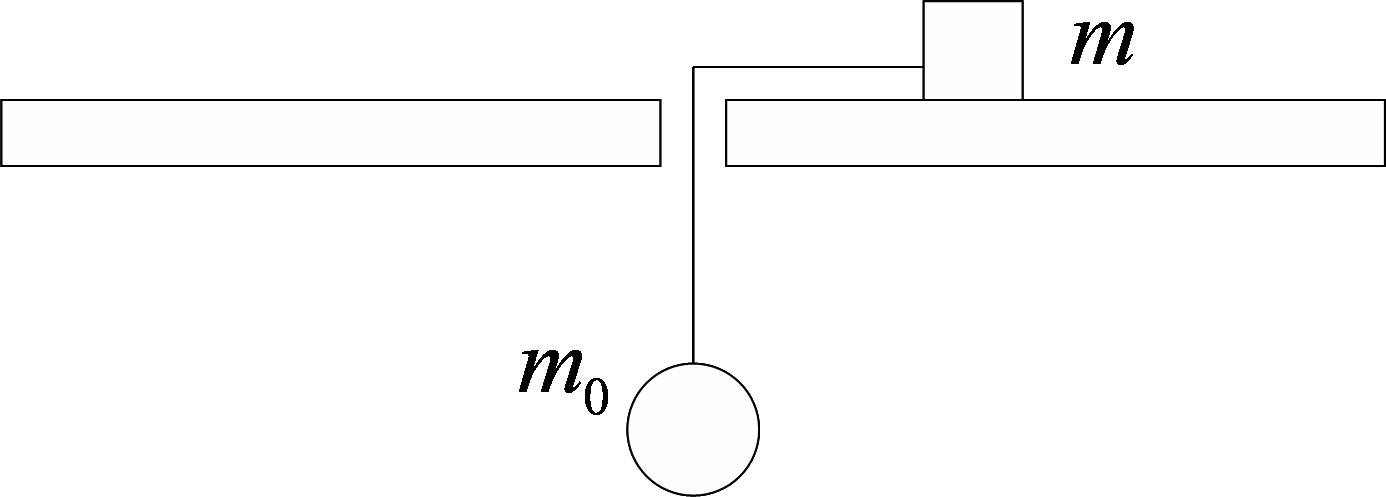
\includegraphics[width=0.4\textwidth, angle=0]{dyn/exercises/massa_op_tafel}
\end{center}
\end{figure}

\end{exercise}

\begin{exercise} Een blokje op een wrijvingsloze tafel beschrijft een ECB met frequentie $f$ en snelheid $v$ doordat het
vastgemaakt is aan een koordje dat door een gaatje in de tafel gaat en waaraan een massa is verbonden die door de zwaartekracht naar beneden wordt getrokken. Hoeveel maal groter is de snelheid van het blokje als het met een tweemaal zo grote frequentie ronddraait? Toon je antwoord aan.
\begin{figure}[!h]
\begin{center}
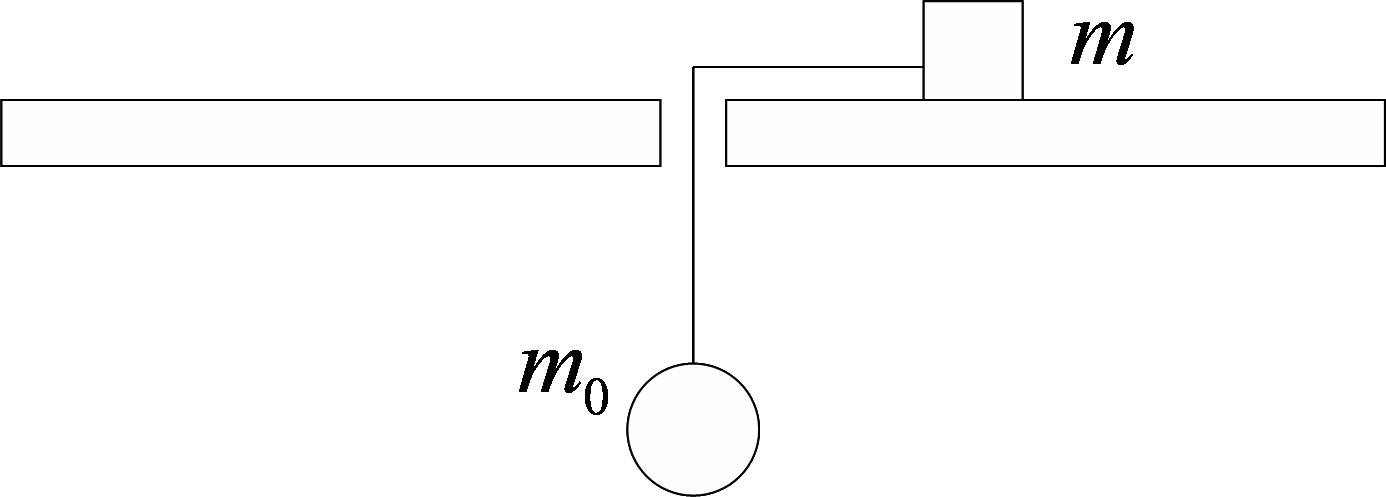
\includegraphics[width=0.4\textwidth, angle=0]{dyn/exercises/massa_op_tafel}
\end{center}
\end{figure}



\end{exercise}

\begin{exercise} Twee treinen met dezelfde massa nemen een bocht met een even grote straal. De snelheden zijn respectievelijk $60~\rm km/h$ en
$180~\rm km/h$ in de bocht.
\begin{enumerate}
\item \textit{Wat} levert de middelpuntzoekende kracht? Op
\textit{wat}?
\item Hoe verhouden de grootten van de middelpuntzoekende kracht zich?
\end{enumerate}


\end{exercise}

\end{document}